\documentclass{article}
\usepackage{CJKutf8}
\usepackage{amsmath}
\usepackage{amssymb}
\usepackage{amsfonts}
\usepackage{amsthm}
\usepackage{titlesec}
\usepackage{titletoc}
\usepackage{xCJKnumb}
\usepackage{tikz}
\titleformat{\chapter}{\centering\Huge\bfseries}{第\, \xCJKnumber{\thechapter}\,
    章}{1em}{}
  % \renewcommand{\chaptermark}[1]{\markboth{第 \thechapter 章}{}}
\usepackage{mathrsfs}

\newtheorem{Def}{定义}
\newtheorem{Thm}{定理}
\newtheorem*{Exercise}{习题}

\newtheorem*{Example}{例}


\begin{document}
\begin{CJK*}{UTF8}{gbsn}
    \begin{Example}
      $X=\{-1,0,1\}$,$Y=\{0,1,2\}$,

      $\forall x \in X, f(x)=x^2$,即$f(-1)=1,f(0)=0,f(1)=1$
  \end{Example}

  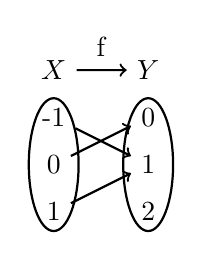
\begin{tikzpicture}[thick, scale=0.3]
  \draw (-2,0) ellipse [x radius=30pt, y radius=80pt];
  \draw (2,0) ellipse [x radius=30pt, y radius=80pt];
  \node[thick] (A) at (-2, 4) {$X$};
  \node[thick] (B) at (2,4) {$Y$};
  \draw[thick, ->] (A) to  (B);

  
  \node[thick] (C) at (-2,2) {-1};
   \node[thick] (D) at  (2,2) {0};

  
  \node[thick] (E) at (-2,0) {0};
  \node[thick] (F) at (2,0) {1};

    \node[thick] (G) at (-2,-2) {1};
    \node[thick] (H) at (2,-2) {2};

    
\draw[thick, ->] (C) to  (F);
\draw[thick, ->] (E) to  (D);
\draw[thick, ->] (G) to  (F);

\draw (0,5) node {f};
\end{tikzpicture}

对$X$的每一个元素$x$,存在唯一的一个$y\in Y$,使得$(x,y) \in f$

  \begin{Example}
    $X=\{-1,0,1\}$,$Y=\{0,1,2\}$,

$f\subseteq X \times Y$,$f=\{(-1,1),(0,0),(1,1)\}$
  \end{Example}

  \begin{Exercise}
    设$X=\{0,1,2\}, Y= \{3,4,5\}, f\subseteq X \times Y$,则下列为映射的是(D)

    A. $f = \{(0,3), (1,4)\}$

    B. $f = \{(0,3), (0,4), (1,4),(2,5)\}$

    C. $f = \{(0,3), (0,4)\}$

    D. $f = \{(0,5), (1,4), (2,3)\}$
  \end{Exercise}

  映射定义的符号化表示:

  $f:X\to Y$
  
  $f\subseteq X\times Y$

  1) $\forall x \in X \exists y (x,y) \in f$

  即:$\forall x x \in X \to \exists y (x,y) \in f$

  2) $\forall x \in X \forall y \in Y ((x,y) \in f \land (x, y') \in f \to y = y')$

  即:$\forall x x \in X \to (\forall y y \in Y \to ((x,y) \in f \land (x, y') \in f \to y = y'))$
    
  
  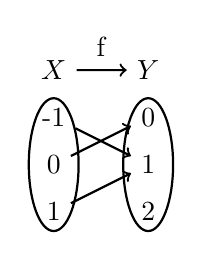
\begin{tikzpicture}[thick, scale=0.3]
  \draw (-2,0) ellipse [x radius=30pt, y radius=80pt];
  \draw (2,0) ellipse [x radius=30pt, y radius=80pt];
  \node[thick] (A) at (-2, 4) {$X$};
  \node[thick] (B) at (2,4) {$Y$};
  \draw[thick, ->] (A) to  (B);

  
  \node[thick] (C) at (-2,2) {-1};
   \node[thick] (D) at  (2,2) {0};

  
  \node[thick] (E) at (-2,0) {0};
  \node[thick] (F) at (2,0) {1};

    \node[thick] (G) at (-2,-2) {1};
    \node[thick] (H) at (2,-2) {2};

    
\draw[thick, ->] (C) to  (F);
\draw[thick, ->] (E) to  (D);
\draw[thick, ->] (G) to  (F);

\draw (0,5) node {f};
\end{tikzpicture}

$f(-1) = 1$

$f$的定义域:$X={-1,0,1}$

$f$的值域:$Im(f) = \{0,1\}$

P(x):x为偶数

$P:Z\to \{T,F\}$

$P\subseteq Z \times \{T,F\}$

$P=\{\ldots, (-2, T), (-1, F), (0, T), (1,F), (2,T), \ldots\}$


  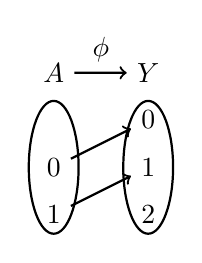
\begin{tikzpicture}[thick, scale=0.3]
  \draw (-2,0) ellipse [x radius=30pt, y radius=80pt];
  \draw (2,0) ellipse [x radius=30pt, y radius=80pt];
  \node[thick] (A) at (-2, 4) {$A$};
  \node[thick] (B) at (2,4) {$Y$};
  \draw[thick, ->] (A) to  (B);

  
%  \node[thick] (C) at (-2,2) {-1};
   \node[thick] (D) at  (2,2) {0};

  
  \node[thick] (E) at (-2,0) {0};
  \node[thick] (F) at (2,0) {1};

    \node[thick] (G) at (-2,-2) {1};
    \node[thick] (H) at (2,-2) {2};

    
%\draw[thick, ->] (C) to  (F);
\draw[thick, ->] (E) to  (D);
\draw[thick, ->] (G) to  (F);

\draw (0,5) node {$\phi$};
\end{tikzpicture}

一个部分映射的例子:

  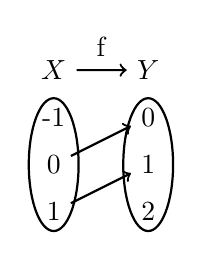
\begin{tikzpicture}[thick, scale=0.3]
  \draw (-2,0) ellipse [x radius=30pt, y radius=80pt];
  \draw (2,0) ellipse [x radius=30pt, y radius=80pt];
  \node[thick] (A) at (-2, 4) {$X$};
  \node[thick] (B) at (2,4) {$Y$};
  \draw[thick, ->] (A) to  (B);

  
  \node[thick] (C) at (-2,2) {-1};
   \node[thick] (D) at  (2,2) {0};

  
  \node[thick] (E) at (-2,0) {0};
  \node[thick] (F) at (2,0) {1};

    \node[thick] (G) at (-2,-2) {1};
    \node[thick] (H) at (2,-2) {2};

    
%\draw[thick, ->] (C) to  (F);
\draw[thick, ->] (E) to  (D);
\draw[thick, ->] (G) to  (F);

\draw (0,5) node {f};
\end{tikzpicture}

一个恒等映射的例子:

  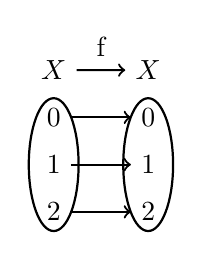
\begin{tikzpicture}[thick, scale=0.3]
  \draw (-2,0) ellipse [x radius=30pt, y radius=80pt];
  \draw (2,0) ellipse [x radius=30pt, y radius=80pt];
  \node[thick] (A) at (-2, 4) {$X$};
  \node[thick] (B) at (2,4) {$X$};
  \draw[thick, ->] (A) to  (B);

  
  \node[thick] (C) at (-2,2) {0};
   \node[thick] (D) at  (2,2) {0};

  
  \node[thick] (E) at (-2,0) {1};
  \node[thick] (F) at (2,0) {1};

    \node[thick] (G) at (-2,-2) {2};
    \node[thick] (H) at (2,-2) {2};

    
\draw[thick, ->] (C) to  (D);
\draw[thick, ->] (E) to  (F);
\draw[thick, ->] (G) to  (H);

\draw (0,5) node {f};
\end{tikzpicture}

一个单射的例子:

  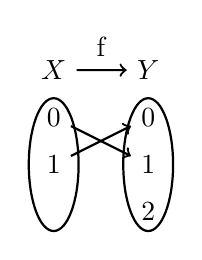
\begin{tikzpicture}[thick, scale=0.3]
  \draw (-2,0) ellipse [x radius=30pt, y radius=80pt];
  \draw (2,0) ellipse [x radius=30pt, y radius=80pt];
  \node[thick] (A) at (-2, 4) {$X$};
  \node[thick] (B) at (2,4) {$Y$};
  \draw[thick, ->] (A) to  (B);

  
  \node[thick] (C) at (-2,2) {0};
   \node[thick] (D) at  (2,2) {0};

  
  \node[thick] (E) at (-2,0) {1};
  \node[thick] (F) at (2,0) {1};

%    \node[thick] (G) at (-2,-2) {2};
    \node[thick] (H) at (2,-2) {2};

    
\draw[thick, ->] (C) to  (F);
\draw[thick, ->] (E) to  (D);
%\draw[thick, ->] (G) to  (H);

\draw (0,5) node {f};
\end{tikzpicture}

一个满射的例子:

  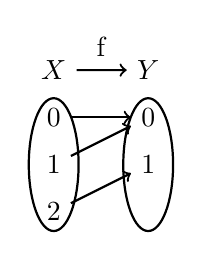
\begin{tikzpicture}[thick, scale=0.3]
  \draw (-2,0) ellipse [x radius=30pt, y radius=80pt];
  \draw (2,0) ellipse [x radius=30pt, y radius=80pt];
  \node[thick] (A) at (-2, 4) {$X$};
  \node[thick] (B) at (2,4) {$Y$};
  \draw[thick, ->] (A) to  (B);

  
  \node[thick] (C) at (-2,2) {0};
   \node[thick] (D) at  (2,2) {0};

  
  \node[thick] (E) at (-2,0) {1};
  \node[thick] (F) at (2,0) {1};

    \node[thick] (G) at (-2,-2) {2};
%    \node[thick] (H) at (2,-2) {2};

    
\draw[thick, ->] (C) to  (D);
\draw[thick, ->] (E) to  (D);
\draw[thick, ->] (G) to  (F);

\draw (0,5) node {f};
\end{tikzpicture}

一个双射的例子:

  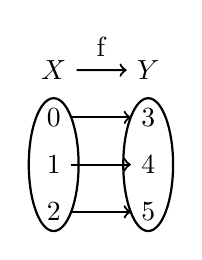
\begin{tikzpicture}[thick, scale=0.3]
  \draw (-2,0) ellipse [x radius=30pt, y radius=80pt];
  \draw (2,0) ellipse [x radius=30pt, y radius=80pt];
  \node[thick] (A) at (-2, 4) {$X$};
  \node[thick] (B) at (2,4) {$Y$};
  \draw[thick, ->] (A) to  (B);

  
  \node[thick] (C) at (-2,2) {0};
   \node[thick] (D) at  (2,2) {3};

  
  \node[thick] (E) at (-2,0) {1};
  \node[thick] (F) at (2,0) {4};

    \node[thick] (G) at (-2,-2) {2};
    \node[thick] (H) at (2,-2) {5};

    
\draw[thick, ->] (C) to  (D);
\draw[thick, ->] (E) to  (F);
\draw[thick, ->] (G) to  (H);

\draw (0,5) node {f};
\end{tikzpicture}

单射的符号化表示:

$f:X\to Y$

$\forall x1 \in X \forall x2 \in X x1 \neq x2 \to f(x1) \neq f(x2)$

即:$\forall x1 \in X \forall x2 \in X  f(x1) = f(x2) \to x1 = x2 $


满射的符号化表示:

$f:X\to Y$

$\forall y \in Y \exists x \in X f(x) = y$


$\{2,3\}^{\{0,1\}} = \{\{(0,2),(1,2)\},\{(0,3),(1,3)\},\{(0,2),(1,3)\},\{(0,3),(1,2)\}\}$

一般的,当$|X| = m$,$|Y| = n$时,

从集合$X$到集合$Y$的映射的个数为$|Y^X|=n^m$

当$n\geq m$时,从集合$X$到集合$Y$的单射的个数为$C_n^mm!$

从集合$X$到集合$Y$的满射的个数?

设$Y=\{y_1,y_2,\ldots, y_n\}$,$A_i=\{f:X\to Y| \forall x \in X f(x) \neq y_i\}$,

则从$X$到$Y$的满射的个数为
\begin{equation*}
  \begin{split}
&n^m - |A_1 \cup A_2 \cup \ldots \cup A_n|\\
=&n^m - (\sum_{i=1}^n|A_i| - \sum_{1\leq i < j \leq n}|A_i \cap A_j| + \sum_{1 \leq  i < j < k \leq n}|A_i \cap A_j \cap A_k|\\
-&\ldots\\
+&(-1)^{n+1}|A_1 \cap A_2 \cap \cdots \cap A_n|)\\
=&n^m - (C_n^1(n-1)^m - C_n^2(n-2)^m + C_n^3(n-3)^m - \ldots + (-1)^nC_n^{n-1}1^m)\\
=&n^m - C_n^1(n-1)^m + C_n^2(n-2)^m - C_n^3(n-3)^m - \ldots + (-1)^{n-1}C_n^{n-1}1^m\\
=&n^m + \sum_{i=1}^{n-1}C_n^i(n-i)^m\\
=&\sum_{i=0}^{n-1}C_n^i(n-i)^m\\
\end{split}
\end{equation*}
 



士兵站队问题:

5 9 10 4 7 2 8 3 6 1

3 2 1  3 2 3 1 2 1 1

\begin{proof}[答]
  用这个垫圈可以盖住$650$个点中的至少$10$个点。以圆内的650个点中的每个点为圆心放一个圆环,则所有圆环的面积之和为$S_1 = 650 * \pi * (3^2 - 2^2) = 3250\pi$。所有圆环所覆盖的区域被包含在一个面积为$\pi * (16 + 3)^2= 361\pi$的圆$C$内。此时必存在$10$个圆环$R_1,R_2,\ldots, R_{10}$有公共的重叠区域,否则所有圆环的面积之和$S_1$将小于圆$C$之面积的$9$倍,即$3250\pi < 9 * 361\pi = 3249\pi$,矛盾。任取圆环$R_1,R_2,\ldots, R_{10}$的公共重叠区域中的一点,在该点上放一个圆环,将覆盖住$R_1,R_2,\ldots,R_{10}$的圆心,这些$10$个圆心都是圆内$650$个点中的点,结论得证。 
\end{proof}


\clearpage

  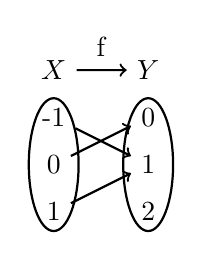
\begin{tikzpicture}[thick, scale=0.3]
  \draw (-2,0) ellipse [x radius=30pt, y radius=80pt];
  \draw (2,0) ellipse [x radius=30pt, y radius=80pt];
  \node[thick] (A) at (-2, 4) {$X$};
  \node[thick] (B) at (2,4) {$Y$};
  \draw[thick, ->] (A) to  (B);

  
  \node[thick] (C) at (-2,2) {-1};
   \node[thick] (D) at  (2,2) {0};

  
  \node[thick] (E) at (-2,0) {0};
  \node[thick] (F) at (2,0) {1};

    \node[thick] (G) at (-2,-2) {1};
    \node[thick] (H) at (2,-2) {2};

    
\draw[thick, ->] (C) to  (F);
\draw[thick, ->] (E) to  (D);
\draw[thick, ->] (G) to  (F);

\draw (0,5) node {f};
\end{tikzpicture}

\begin{equation*}
  \begin{split}
    &f^{-1}(\{0,1\}\cup \{1,2\})\\
    =&f^{-1}(\{0,1,2\})\\
    =&\{-1,0,1\}\\
    &f^{-1}(\{0,1\})\cup f^{-1}(\{1,2\})\\
    =&\{0,-1,1\}\cup \{-1,1\}\\
    =&\{0,-1,1\}
  \end{split}
\end{equation*}

$f^{-1}(C \cup D) = f^{-1}(C) \cup f^{-1}(D)$
\begin{equation*}
  \begin{split}
    \forall x \in X &x\in f^{-1}(C \cup D)\\
    &\Leftrightarrow f(x) \in C \cup D\\
    &\Leftrightarrow f(x) \in C \lor f(x) \in D\\
    &\Leftrightarrow x \in f^{-1}(C) \lor x \in f^{-1}(D)\\
    &\Leftrightarrow x \in f^{-1}(C) \cup f^{-1}(D)\\
  \end{split}
\end{equation*}
\begin{proof}[证明]
  先证$f^{-1}(C \cup D) \subseteq f^{-1}(C) \cup f^{-1}(D)$:
  
  对任意的$x\in X$,如果$x\in f^{-1}(C \cup D)$,则$f(x) \in C \cup D$,从而$f(x) \in C$ 或者 $f(x) \in D$,于是$x \in f^{-1}(C)$ 或者 $x \in f^{-1}(D)$,因此$x\in x \in f^{-1}(C) \cup f^{-1}(D)$。
  
  再证$f^{-1}(C) \cup f^{-1}(D)\subseteq f^{-1}(C \cup D)$:

  对任意的$x\in X$,如果$x\in f^{-1}(C) \cup f^{-1}(D)$,则$x\in f^{-1}(C)$或者$x \in f^{-1}(D)$,从而$f(x) \in C$或者$f(x) \in D$,于是$f(x) \in C \cup D$,因此$x\in f^{-1}(C \cup D)$。
\end{proof}
  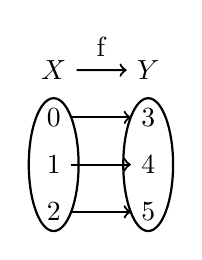
\begin{tikzpicture}[thick, scale=0.3]
  \draw (-2,0) ellipse [x radius=30pt, y radius=80pt];
  \draw (2,0) ellipse [x radius=30pt, y radius=80pt];
  \node[thick] (A) at (-2, 4) {$X$};
  \node[thick] (B) at (2,4) {$Y$};
  \draw[thick, ->] (A) to  (B);

  
  \node[thick] (C) at (-2,2) {0};
   \node[thick] (D) at  (2,2) {3};

  
  \node[thick] (E) at (-2,0) {1};
  \node[thick] (F) at (2,0) {4};

    \node[thick] (G) at (-2,-2) {2};
    \node[thick] (H) at (2,-2) {5};

    
\draw[thick, ->] (C) to  (D);
\draw[thick, ->] (E) to  (F);
\draw[thick, ->] (G) to  (H);

\draw (0,5) node {f};
\end{tikzpicture}\hspace{1cm}

\clearpage
  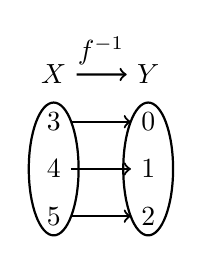
\begin{tikzpicture}[thick, scale=0.3]
  \draw (-2,0) ellipse [x radius=30pt, y radius=80pt];
  \draw (2,0) ellipse [x radius=30pt, y radius=80pt];
  \node[thick] (A) at (-2, 4) {$X$};
  \node[thick] (B) at (2,4) {$Y$};
  \draw[thick, ->] (A) to  (B);

  
  \node[thick] (C) at (-2,2) {3};
   \node[thick] (D) at  (2,2) {0};

  
  \node[thick] (E) at (-2,0) {4};
  \node[thick] (F) at (2,0) {1};

    \node[thick] (G) at (-2,-2) {5};
    \node[thick] (H) at (2,-2) {2};

    
\draw[thick, ->] (C) to  (D);
\draw[thick, ->] (E) to  (F);
\draw[thick, ->] (G) to  (H);

\draw (0,5) node {$f^{-1}$};
\end{tikzpicture}

$X=\{0,1,2\}, Y = \{3,4,5\}, f:X\to Y f(0) = 3, f(1) = 4, f(2) = 5$ \hspace{1cm} $f^{-1}:Y\to X f^{-1}(3) = 0, f^{-1}(4) = 1, f^{-1}(5) = 2$

$X=\{0,1,2\}, Y = \{3,4,5\}, f:X\to Y f=\{(0,3),(1,4),(2,5)\}$ \hspace{1cm} $f^{-1}:Y\to X f^{-1}=\{(3,0),(4,1),(5,2)\}$

 \begin{Thm}
    设$f:X\to Y$为可逆映射,则$(f^{-1})^{-1}=f$。
  \end{Thm}
  \begin{proof}[证法一]
    因为$f\circ f^{-1}=I_{Y}$并且$f^{-1}\circ f=I_X$,由逆映射的定义知,$f^{-1}$的逆映射为$f$,所以$(f^{-1})^{-1}=f$。
  \end{proof}
  \begin{proof}[证法二]
    \begin{equation*}
      \begin{split}
        \forall x\in X \forall y\in Y &(x,y) \in (f^{-1})^{-1}\\
        \Leftrightarrow &(y,x) \in f^{-1}\\
        \Leftrightarrow &(x,y) \in f
      \end{split}
    \end{equation*}
  \end{proof}

  \begin{Thm}
    设$f:X\to Y$,$g:Y\to Z$都为可逆映射,则$g\circ f$也为可逆映射并且$(g\circ f)^{-1} = f^{-1}\circ g^{-1}$。
  \end{Thm}

  \begin{proof}[证明]
    可以验证:
    \begin{align*}
      &(gf)(f^{-1}g^{-1})=g(ff^{-1})g^{-1}=gg^{-1}=I_Z\\
      &(f^{-1}g^{-1})gf = f^{-1}(g^{-1}g)f=f^{-1}f= I_X
    \end{align*}
    因此$(gf)^{-1}=f^{-1}g^{-1}$。
  \end{proof}


  一个左逆映射的例子:
  
  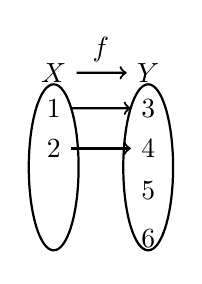
\begin{tikzpicture}[thick, scale=0.3]
  \draw (-2,0) ellipse [x radius=30pt, y radius=100pt];
  \draw (2,0) ellipse [x radius=30pt, y radius=100pt];
  \node[thick] (A) at (-2, 4) {$X$};
  \node[thick] (B) at (2,4) {$Y$};
  \draw[thick, ->] (A) to  (B);

  
  \node[thick] (C) at (-2,2.5) {1};
   \node[thick] (D) at  (2,2.5) {3};

  
  \node[thick] (E) at (-2,0.8) {2};
  \node[thick] (F) at (2,0.8) {4};

    \node[thick] (G) at (2,-1) {5};
    \node[thick] (H) at (2,-3) {6};

    
\draw[thick, ->] (C) to  (D);
\draw[thick, ->] (E) to  (F);

\draw (0,5) node {$f$};
\end{tikzpicture}\hspace{1cm}
  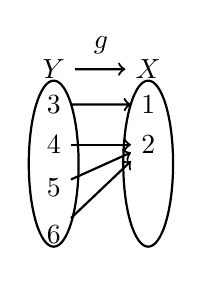
\begin{tikzpicture}[thick, scale=0.3]
  \draw (-2,0) ellipse [x radius=30pt, y radius=100pt];
  \draw (2,0) ellipse [x radius=30pt, y radius=100pt];
  \node[thick] (A) at (-2, 4) {$Y$};
  \node[thick] (B) at (2,4) {$X$};
  \draw[thick, ->] (A) to  (B);

  
  \node[thick] (C) at (2,2.5) {1};
   \node[thick] (D) at  (-2,2.5) {3};

  
  \node[thick] (E) at (2,0.8) {2};
  \node[thick] (F) at (-2,0.8) {4};

    \node[thick] (G) at (-2,-1) {5};
    \node[thick] (H) at (-2,-3) {6};

    
\draw[thick, ->] (D) to  (C);
\draw[thick, ->] (F) to  (E);
\draw[thick, ->] (G) to  (E);
\draw[thick, ->] (H) to  (E);

\draw (0,5) node {$g$};
\end{tikzpicture}



  一个右逆映射的例子:
  
  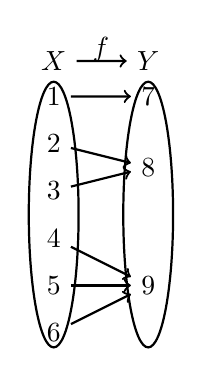
\begin{tikzpicture}[thick, scale=0.3]
  \draw (-2,0) ellipse [x radius=30pt, y radius=160pt];
  \draw (2,0) ellipse [x radius=30pt, y radius=160pt];
  \node[thick] (A) at (-2, 6.5) {$X$};
  \node[thick] (B) at (2,6.5) {$Y$};
  \draw[thick, ->] (A) to  (B);

  
  \node[thick] (C) at (-2,5) {1};
   \node[thick] (D) at  (-2,3) {2};

  
  \node[thick] (E) at (-2,1) {3};
  \node[thick] (F) at (-2,-1) {4};

    \node[thick] (G) at (-2,-3) {5};
    \node[thick] (H) at (-2,-5) {6};

        \node[thick] (I) at (2,5) {7};
    \node[thick] (J) at (2,2) {8};
    \node[thick] (K) at (2,-3) {9};

    
\draw[thick, ->] (C) to  (I);
\draw[thick, ->] (D) to  (J);
\draw[thick, ->] (E) to  (J);
\draw[thick, ->] (F) to  (K);
\draw[thick, ->] (G) to  (K);
\draw[thick, ->] (H) to  (K);

\draw (0,7) node {$f$};
\end{tikzpicture}\hspace{1cm}
  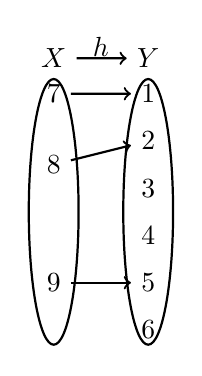
\begin{tikzpicture}[thick, scale=0.3]
  \draw (-2,0) ellipse [x radius=30pt, y radius=160pt];
  \draw (2,0) ellipse [x radius=30pt, y radius=160pt];
  \node[thick] (A) at (-2, 6.5) {$X$};
  \node[thick] (B) at (2,6.5) {$Y$};
  \draw[thick, ->] (A) to  (B);

  
  \node[thick] (C) at (2,5) {1};
   \node[thick] (D) at  (2,3) {2};

  
  \node[thick] (E) at (2,1) {3};
  \node[thick] (F) at (2,-1) {4};

    \node[thick] (G) at (2,-3) {5};
    \node[thick] (H) at (2,-5) {6};

        \node[thick] (I) at (-2,5) {7};
    \node[thick] (J) at (-2,2) {8};
    \node[thick] (K) at (-2,-3) {9};

    
\draw[thick, ->] (I) to  (C);
\draw[thick, ->] (J) to  (D);
\draw[thick, ->] (K) to  (G);

\draw (0,7) node {$h$};
\end{tikzpicture}

$f$左可逆 $\Rightarrow f$单:

$f:X\to Y$单:

$\forall x1 \in X \forall x2 \in X x1 \neq x2 \to f(x1) \neq f(x2)$

即:$\forall x1 \in X \forall x2 \in X  f(x1) = f(x2) \to x1 = x2 $


$gf=I_X$

$\forall x_1\in X$ $\forall x_2\in Y$ 如果$f(x_1)=f(x_2)$,则$gf(x_1)=gf(x_2)$,从而$x_1=x_2$
 
$f$单$\Rightarrow f$左可逆:

$f':X\to Im(f) f'(x) = f(x)$

\begin{equation*}
  g(y)=
  \begin{cases}
    f'^{-1}(y) & y \in Im(f)\\
    x_0 &y \notin Im(f) x_0\text{为}X\text{中任意选定的一个元素}\\
  \end{cases}
\end{equation*}


$f$右可逆$\Rightarrow f$满:


$f:X\to Y$满:

$\forall y \in Y \exists x \in X f(x) = y$

$fh=I_Y$  $\forall y\in Y f(h(y))=y$

$f$满$\Rightarrow f$右可逆

$h(y)=x$ $x$为$f^{-1}({y})$中任意选定的一个元素


  \begin{Example}
    设$S=\{1,2,3\}$,$\alpha$和$\beta$为$S$上的两个置换,
    \[\alpha=\begin{pmatrix}1&2&3\\1&3&2\end{pmatrix},\beta=\begin{pmatrix}1&2&3\\2&3&1\end{pmatrix}\],
    则
    \[\alpha\beta=\begin{pmatrix}1&2&3\\1&3&2\end{pmatrix}\begin{pmatrix}1&2&3\\2&3&1\end{pmatrix}=\begin{pmatrix}1&2&3\\2&1&3\end{pmatrix}\],    
  \end{Example}

  \begin{Example}
    \[\alpha\beta=\begin{pmatrix}1&2&3\\1&3&2\end{pmatrix}\begin{pmatrix}1&2&3\\2&3&1\end{pmatrix}=\begin{pmatrix}1&2&3\\1&3&2\end{pmatrix}\begin{pmatrix}1&3&2\\2&1&3\end{pmatrix}=\begin{pmatrix}1&2&3\\2&1&3\end{pmatrix}\]
            \[\beta\alpha=\begin{pmatrix}1&2&3\\2&3&1\end{pmatrix}\begin{pmatrix}1&2&3\\1&3&2\end{pmatrix}=\begin{pmatrix}1&2&3\\2&3&1\end{pmatrix}\begin{pmatrix}2&3&1\\3&2&1\end{pmatrix}=\begin{pmatrix}1&2&3\\3&2&1\end{pmatrix}\]

      \end{Example}

      

      群:
      
      $(\alpha \beta) \theta = \alpha (\beta \theta)$

      $I\alpha = \alpha I = \alpha$

      $\alpha^{-1}\alpha = \alpha \alpha^{-1} = I$
      
        \begin{Example}
    设$S=\{1,2,3\}$,
    \[I=\begin{pmatrix}1&2&3\\1&2&3\end{pmatrix}\],    
  \end{Example}


  
  \begin{Example}
    设$S=\{1,2,3\}$,
    \[\alpha=\begin{pmatrix}1&2&3\\1&3&2\end{pmatrix}\]
    则
    \[\alpha^{-1}=\begin{pmatrix}1&3&2\\1&2&3\end{pmatrix}=\begin{pmatrix}1&2&3\\1&3&2\end{pmatrix}\]    
  \end{Example}
      
      
         \begin{Example}
   设$S=\{1,2,3,4,5\}$,则$(2,3,5)=\begin{pmatrix}1&2&3&4&5\\1&3&5&4&2\end{pmatrix}$,$(2,3)=\begin{pmatrix}1&2&3&4&5\\1&3&2&4&5\end{pmatrix}$     
   \end{Example}

   数学归纳法I:

   $\forall n P(n)$

   (1)当$n=1$时结论成立 $P(1)$

   (2)假设当$n=k$时结论成立,往证$n=k+1$时结论也成立 $P(k)\to P(k+1)$


   $P(k)$:
   
   如果$A_1\subseteq A_2\subseteq \ldots \subseteq A_{k} \subseteq A_1$, 那么$A_1 = A_2 = \ldots = A_k$。

   $P(k+1)$:

   如果$A_1\subseteq A_2\subseteq \ldots \subseteq A_{k} \subseteq A_{k+1} \subseteq A_1$,那么$A_1=A_2=\ldots = A_k = A_{k+1}$。

   
   数学归纳法II:

   $\forall n P(n)$

   (1)当$n=1$时结论成立 P(1)

   (2)假设当$n<k$时结论成立,往证当$n=k$结论也成立 $(\forall n (n<k\to p(n))) \to p(k)$ 

   \begin{proof}[证明]
     $\sigma = (i_1i_2\ldots i_l)\tau$
   \end{proof}

   \begin{proof}[证明]
     设$A$为所有的$n$次奇置换所构成的集合,$B$为所有的偶置换所构成的集合,则$S_n=A\cup B$且$A\cap B=\phi$。所以,$|S_n|=|A| + |B|=n!$。

     以下证明$|A|=|B|$。构造映射$f:A\to B$,对任意的$\sigma\in A$,$f(\sigma) = \sigma(12)$。易验证$f$为单射,这是因为对任意的$\sigma_1\in A$,$\sigma_2\in A$,如果$f(\sigma_1)=f(\sigma_2)$,则$\sigma_1(1,2)=\sigma_2(1,2)$,从而$\sigma_1(1,2)(1,2)=\sigma_2(1,2)(1,2)$,即$\sigma_1=\sigma_2$。同时,易验证$f$为满射,这是因为对任意的$\tau \in B$,$f(\tau(1,2))=\tau(1,2)(1,2)=\tau$。从而$f$为双射,这证明了$|A|=|B|$。再由$|A|+|B|=n!$知,$|A|=|B|=\frac{n!}{2}$。
   \end{proof}
\end{CJK*}
\end{document}
